\chapter{Introduction}


\section{Overview}

PyLith is portable, scalable software for simulation of crustal
deformation across spatial scales ranging from meters to hundreds of
kilometers and temporal scales ranging from milliseconds to thousands
of years. Its primary applications are quasi-static and dynamic
modeling of earthquake faulting.

\section{New in PyLith Version \pylithVersionNumber}
\begin{itemize}
\item Major rewrite of the finite-element implementation to support
  higher order discretizations and flexible specification of the
  governing equations.
  \begin{itemize}
  \item Use of point-wise functions to implement governing equations;
  \item Higher order discretizations;
  \item Problem specification independent of cell shape (quad vs tri,
    hex vs tet);
  \item Incompressible elasticity;
  \end{itemize}
\item Use of PETSc time-stepping algorithms;
\item New examples
  \begin{itemize}
  \item Simple 2-D and 3-D examples without faults;
  \item Prescribed slip on a 2-D through-going strike-slip fault; and
  \item Prescribed slip on a reverse fault with a splay fault;
  \end{itemize}
\end{itemize}
The \filename{CHANGES} file in the top-level source directory contains
a summary of features and bugfixes for each release.


\section{History}

PyLith 1.0 was the first version to allow the solution of both
implicit (quasi-static) and explicit (dynamic) problems and was a
complete rewrite of the original PyLith (version 0.8). PyLith 1.0
combines the functionality of EqSim
\cite{Aagaard:etal:2001a,Aagaard:etal:2001b} and PyLith 0.8. PyLith
0.8 was a direct descendant of LithoMop and was the first version that
ran in parallel, as well as providing several other improvements over
LithoMop. LithoMop was the product of major reengineering of Tecton, a
finite-element code for simulating static and quasi-static crustal
deformation. The major new features present in LithoMop included
dynamic memory allocation and the use of the Pyre simulation framework
and PETSc solvers. EqSim was written by Brad Aagaard to solve problems
in earthquake dynamics, including rupture propagation and seismic wave
propagation.

The release of PyLith 1.0 has been followed by additional releases
that expand the number of features as well as improve performance.
The PyLith 1.x series of releases allows the solution of both
quasi-static and dynamic problems in one, two, or three
dimensions. The code runs in either serial or parallel, and the design
allows for relatively easy scripting using the Python programming
language. Material properties and values for boundary and fault
conditions are specified using spatial databases, which permit easy
prescription of complex spatial variations of properties and
parameters. Simulation parameters are generally specified through the
use of simple ASCII files or the command line.  At present, mesh
information may be provided using a simple ASCII file (PyLith mesh
ASCII format) or imported from CUBIT or LaGriT, two widely-used
meshing packages. The elements currently available include a linear
bar in 1D, linear triangles and quadrilaterals in 2D, and linear
tetrahedra and hexahedra in 3D. Materials presently available include
isotropic elastic, linear Maxwell viscoelastic, generalized Maxwell
viscoelastic, power-law viscoelastic, and Drucker-Prager
elastoplastic. Boundary conditions include Dirichlet (prescribed
displacements and velocities), Neumann (traction), point forces, and
absorbing boundaries.  Cohesive elements are used to implement slip
across interior surfaces (faults) with both kinematically-specified
fault slip and slip governed by fault constitutive models. PyLith also
includes an interface for computing static Green's functions for fault
slip.

PyLith 2.0 replaces the finite-element data structures provided by the
C++ Sieve implementation with those provided by the C DMPlex
implementation.  The newly developed DMPlex implementation by the
PETSc developers conforms to the PETSc data manager (DM) interface,
thereby providing tighter integration with other PETSc data
structures, such as vectors and matrices. Other improvements include
significantly reduced memory use and memory balancing.

PyLith 3.0 \todo{brad/charles}{Describe changes in v3.0.}

PyLith is under active development and we expect a number of additions
and improvements in the near future. Likely enhancements will include
additional bulk and fault constitutive models, coupled quasi-static
and dynamic simulations for earthquake cycle modeling, and coupling
between elasticity, heat flow, and/or fluid flow.


\section{PyLith Workflow}

PyLith is one component in the process of investigating problems in
tectonics (Figure \vref{fig:Workflow-summary}). Given a geological
problem of interest, a scientist must first provide a geometrical
representation of the desired structure. Once the structure has been
defined, a computational mesh must be created. PyLith presently
provides three mesh importing options: CUBIT Exodus format, LaGriT GMV
and Pset files, and PyLith mesh ASCII format. The modeling of the
physical processes of interest is performed by a code such as
PyLith. Present output consists of VTK or HDF5/Xdmf files which can be
used by a number of visualization codes (e.g., ParaView, Visit, and
Matlab).

\begin{figure}[htbp]
  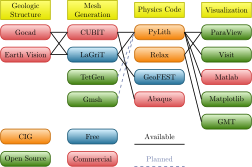
\includegraphics[width=4in]{intro/figs/workflow}
  \caption{Workflow involved in going from geologic structure to
    problem analysis.}
  \label{fig:Workflow-summary}
\end{figure}

